\section{Tools For Painless Object Detection (TPOD)}
\label{sec: app-dev-tpod}

Training a DNN for object detection is not trivial.  In particular, it involves
constructing a correctly-labeled training data set with millions of positive and
negative examples. The training process itself may take days to complete, and
involves a set of arcane procedures to ensure both convergence and efficacy of
the model. Fortunately, one does not typically need to train a DNN from scratch.
Rather, one can start with a pretrained model based on a public image data set
such as ImageNet, and then adapt it to detect custom classes for a new
application, though a process called \emph{transfer learning}.  The key idea is
that much of the training teaches the model to discover low-level features, such
as edges, textures, shapes, and patterns that are useful in distinguishing
objects, and such features can largely be reused in other detection tasks on
similar images.  Thus, adapting a pretrained model for new object classes
requires only thousands of examples and hours of training time. 

However, even with transfer learning, collecting a labeled training set of a
thousand examples per object class can be a daunting and painful task. In
addition, implementing DNNs requires expertise and takes time. TPOD is a
web-based tool we developed to streamline the process of creating DNN-based
object detectors for fast prototype. It provides a tracking-assisted labeling
interface for speedy annotation and transfer learning-based DNN training and
evaluation backends that abstract the nuances of DNNs. It helps to greatly
reduce the labeling effort while constructing the dataset, and automates and
takes some of the guesswork out of training a DNN model.

% A user would first
% upload short videos of the object collected from varying lighting conditions and
% perspectives. Then, the user would label these objects using TPOD's labeling
% interface. TPOD assists labeling by tracking the labeled object across frames.
% Augmenting training data with synthetically generated data is also supported. A
% user then can start training from the web interface. TPOD backend uses transfer
% learning to finetune an object detector DNN from publicly available networks
% that have been trained with millions of images. When the training is done, a
% user can downl.oad the object detector as a container image to run the trained
% models for inference. TPOD also provides interfaces for evaluating and testing
% trained DNNs.

\subsection{Creating a Object Detector with TPOD}

\begin{figure}[]
  \centering
  \begin{minipage}[b]{0.32\textwidth}
    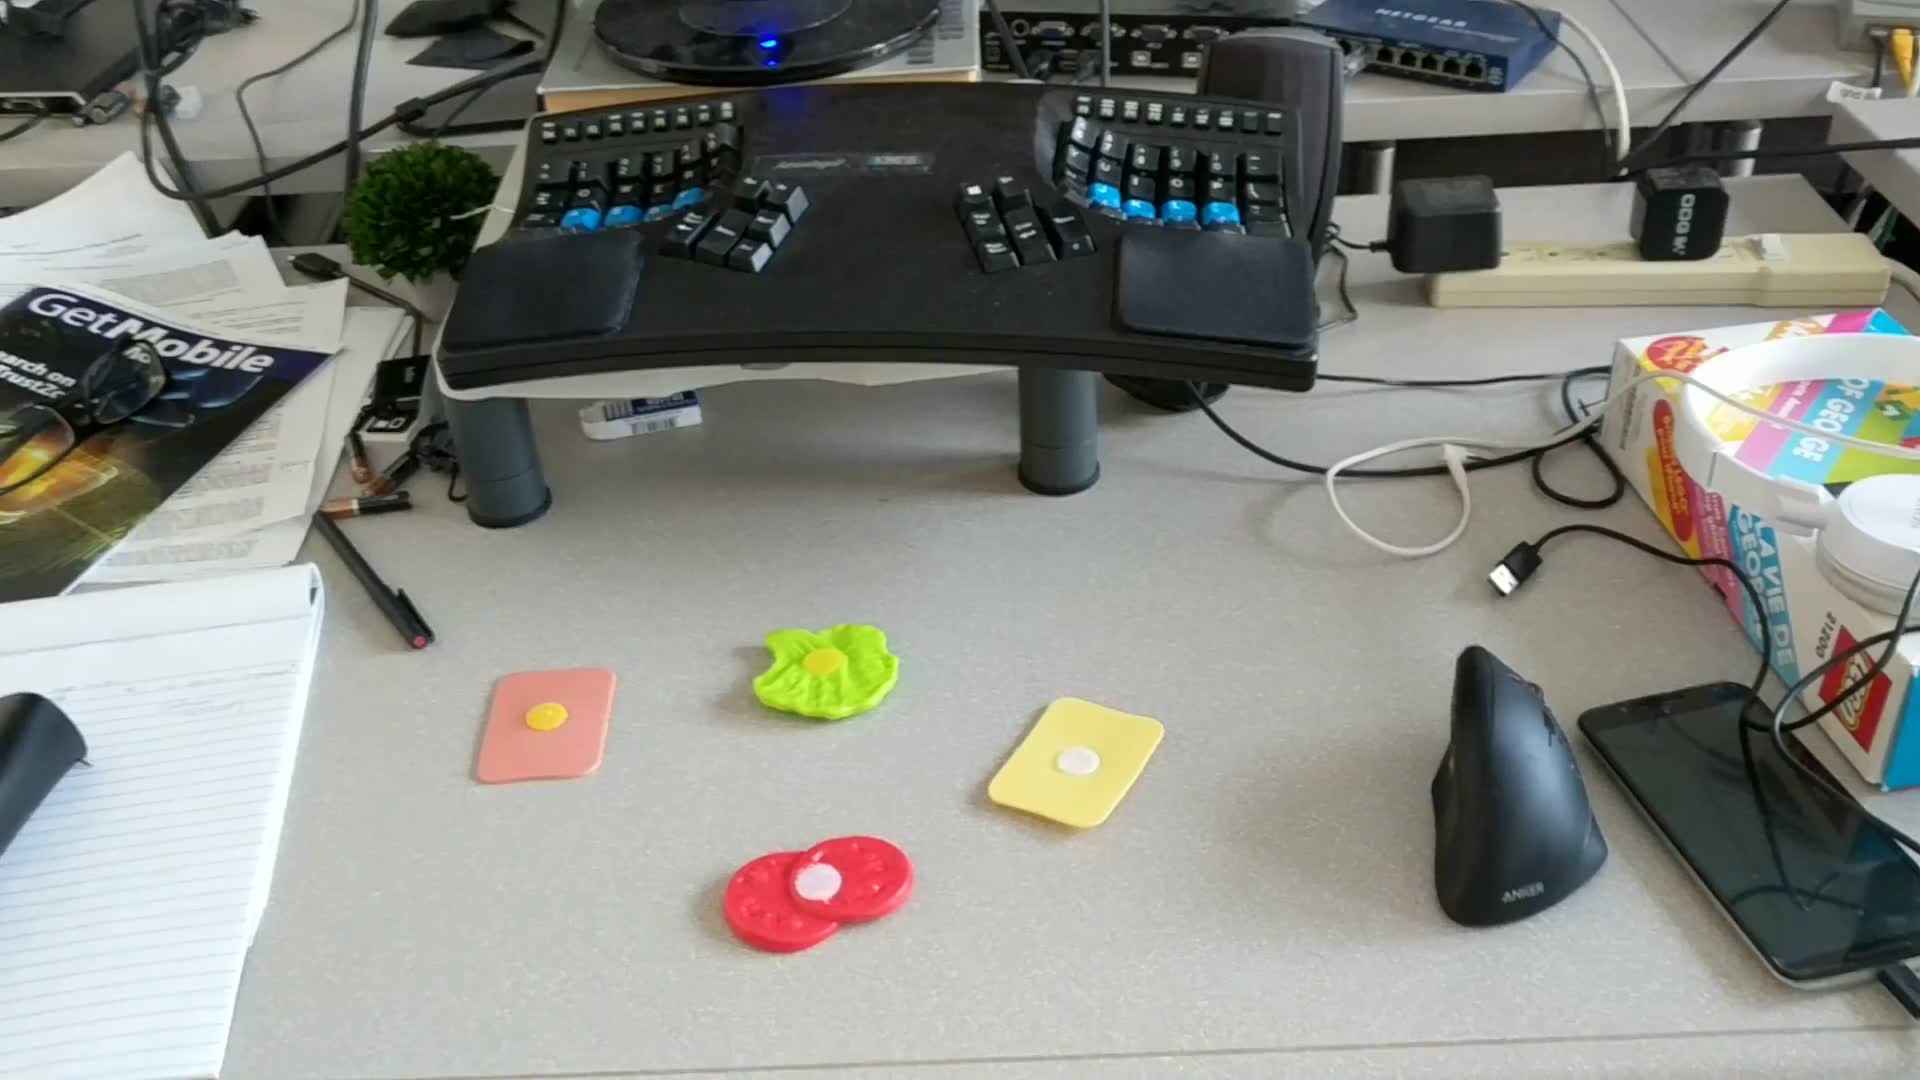
\includegraphics[width=\textwidth]{FIGS/sandwich-training-1.jpg}
  \end{minipage}
  \begin{minipage}[b]{0.32\textwidth}
    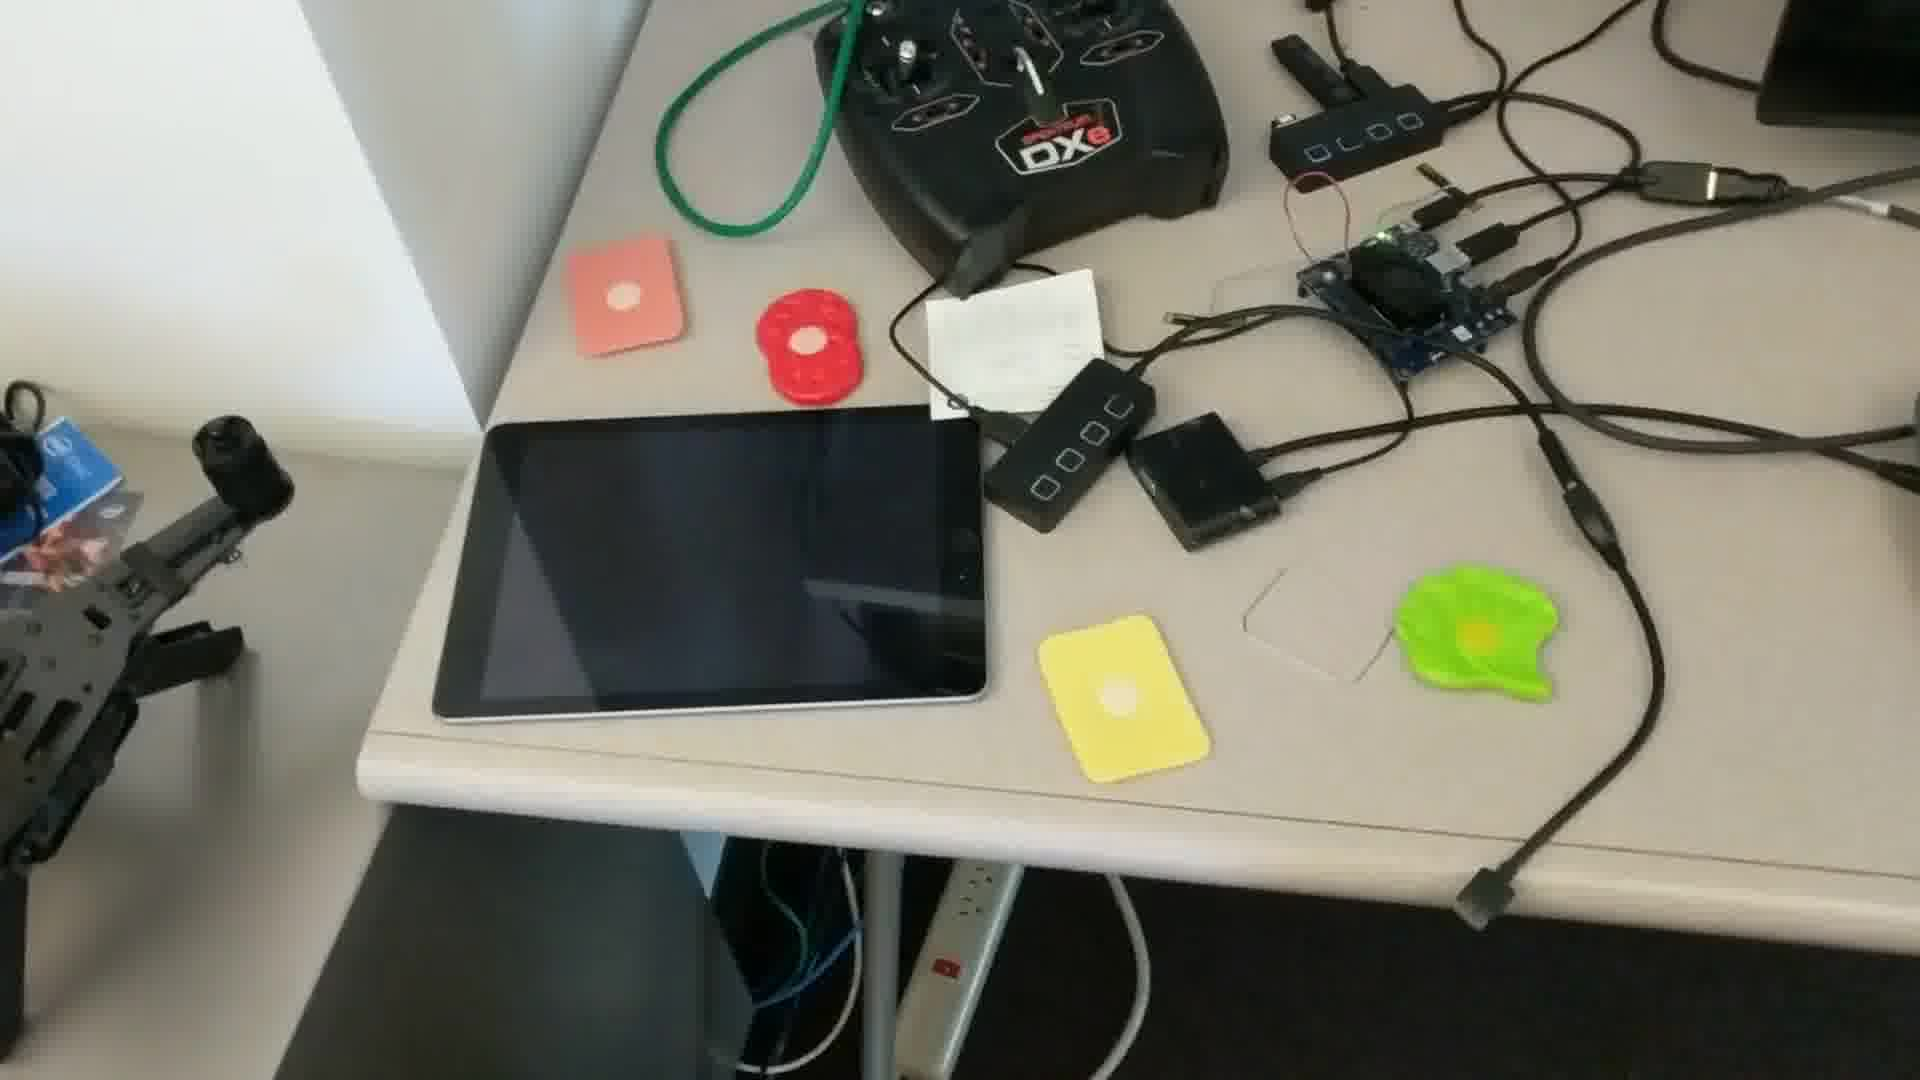
\includegraphics[width=\textwidth]{FIGS/sandwich-training-2.jpg}
  \end{minipage}
  \begin{minipage}[b]{0.32\textwidth}
    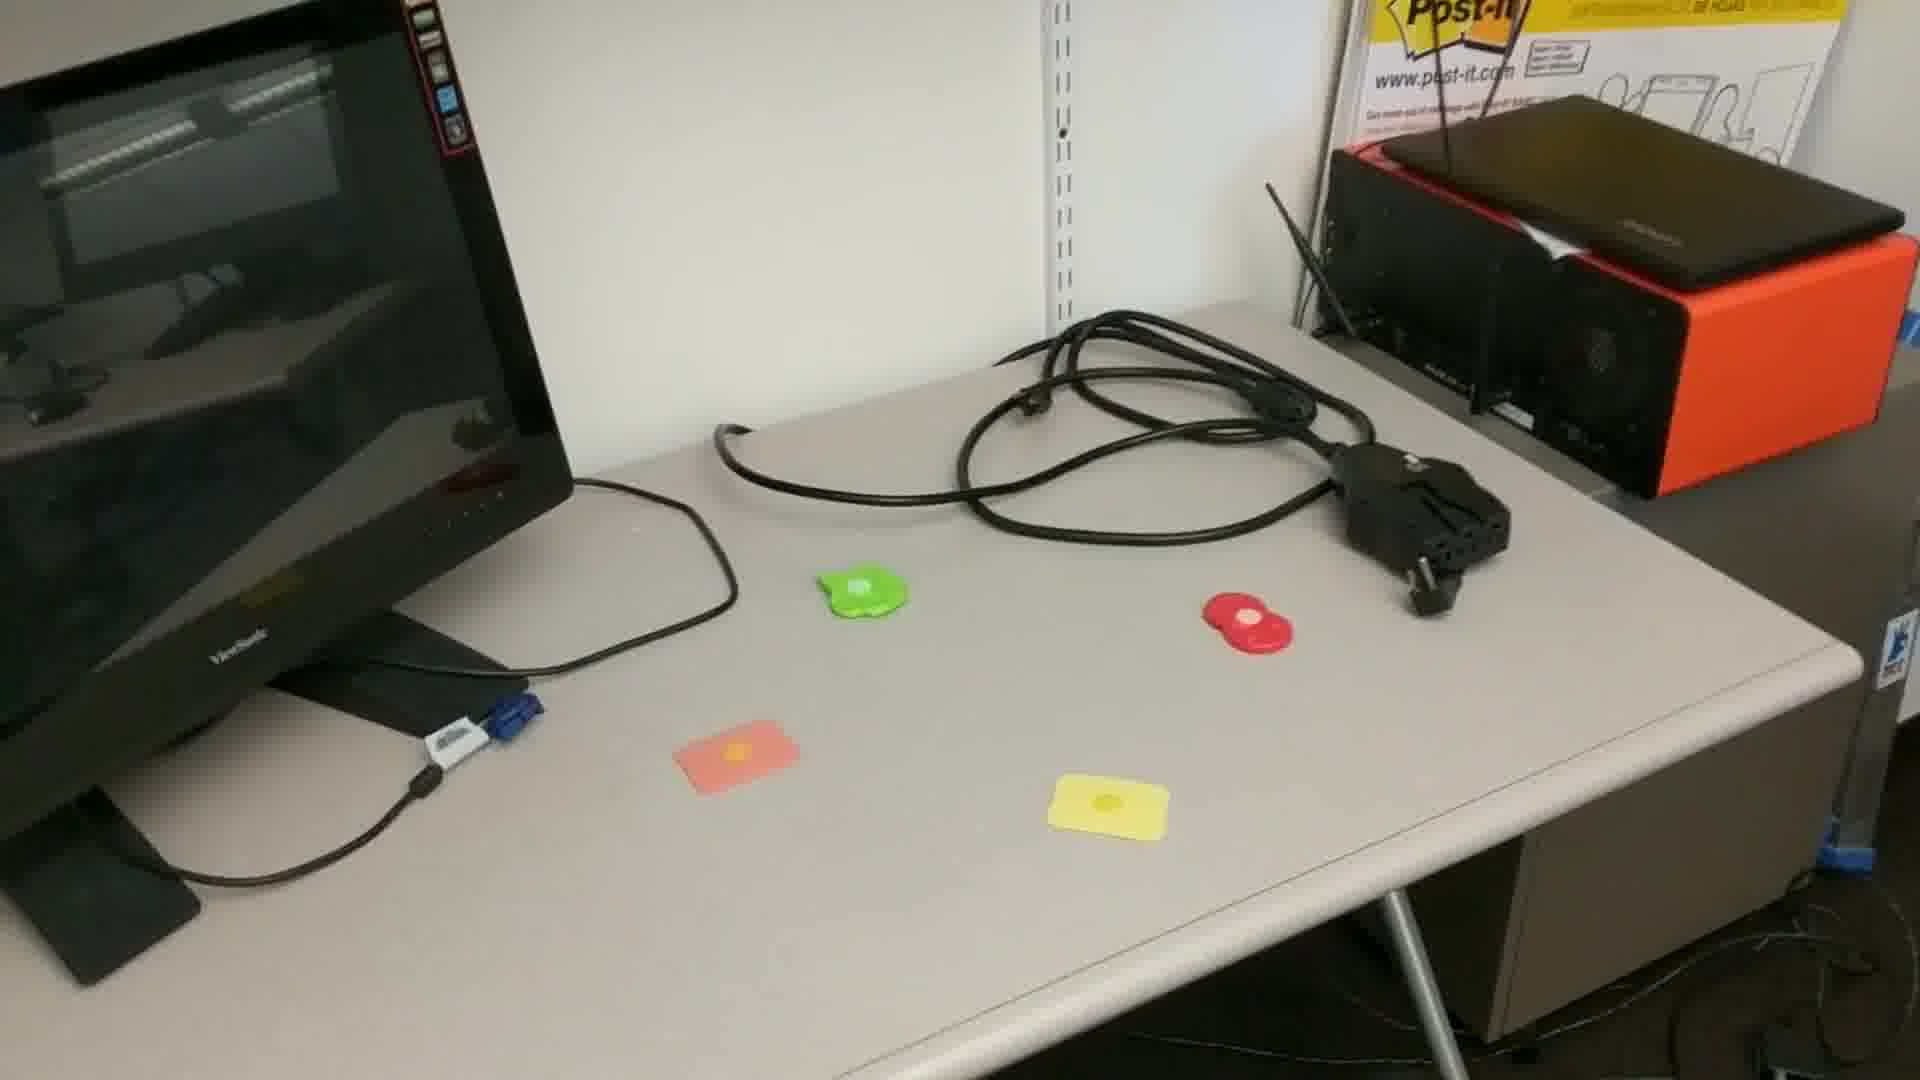
\includegraphics[width=\textwidth]{FIGS/sandwich-training-3.jpg}
  \end{minipage}
    \caption{TPOD Training Images Examples}
  \label{figs:tpod-example-training-images}
\end{figure}

Using TPOD to create object detectors is straight-forward. Developer first
captures videos of objects from various viewing angles and diverse backgrounds.
These videos can be captured on a mobile phone. At 30 frames per second, ten
mintues of video footage contain 18000 frames, which is already an acceptable
amount of training data for transfer learning. An larger amount of training data
typically helps increase the accuracy, although diminishing return also applies.
Moreover, it is preferred to collect training examples similar to the test
environment, as they present more suitable distribution for the model to learn.
Figure~\ref{figs:tpod-example-training-images} shows three example training
images for a toy cooking set. Note that the image background will be used as
negative examples to illustrate to the neural network about what an object does
not look like. Therefore, background better contains common objects in the test
environment that may cause wrong detections.


\begin{figure}[]
  \centering
    \fbox{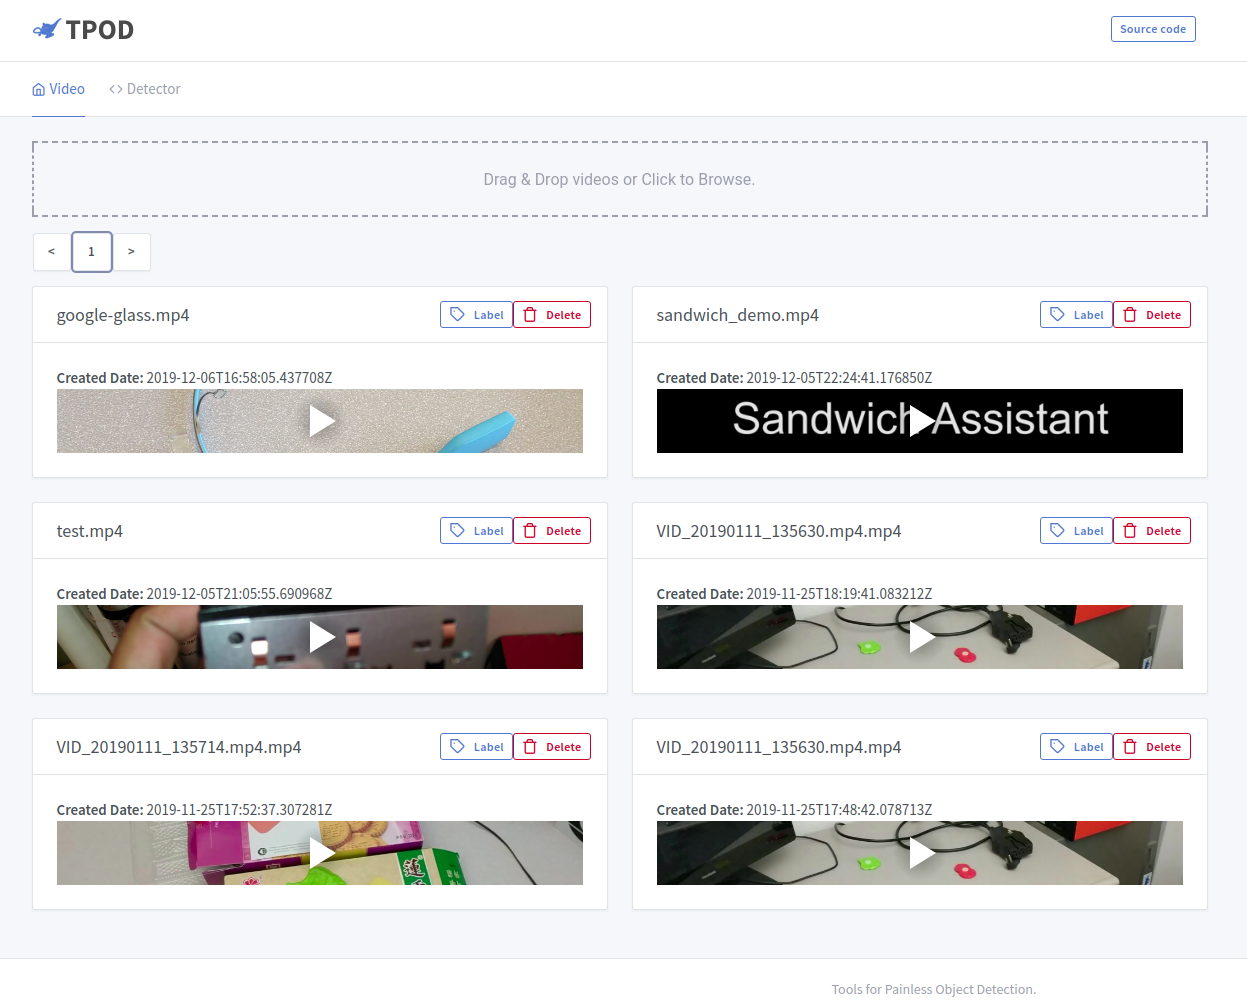
\includegraphics[width=\textwidth]{FIGS/tpod-video-gui}}
    \caption{TPOD Video Management GUI}
  \label{figs:tpod-video-gui}
\end{figure}

Next, developers upload the collected training videos to TPOD either directly
from the phone or from a computer. As shown in Figure~\ref{figs:tpod-video-gui},
TPOD helps user to store and organize training videos. TPOD helps users annotate
the training videos by integrating an external labeling tool into the GUI. Uers
annotate objects of interests by draw bounding boxes on the video frame. To help
facilitate the annotation process, TPOD leverages the fact that the frames are
part of a continuous video shot, and automatically generate bounding box in
subsequent frames using a correlation tracking
algorithm~\cite{danelljan2014accurate}. Therefore, users only need to label a
few key frames in a video with the rest of frames auto-populated with generated
labels. Of course, tracking is not perfect, and the bounding box may drift off
the object over time. In this case, the user can scroll forward or back in the
video, and adjust the bounding box to better match the object.  The adjustment
of bounding boxes reinitializes the tracking for subsequent frames. Overall,
this approach of labeling followed by tracking can reduce the number of frames
that the user needs to manually label by a factor of 10-20x.

\begin{figure}[]
  \centering
    \fbox{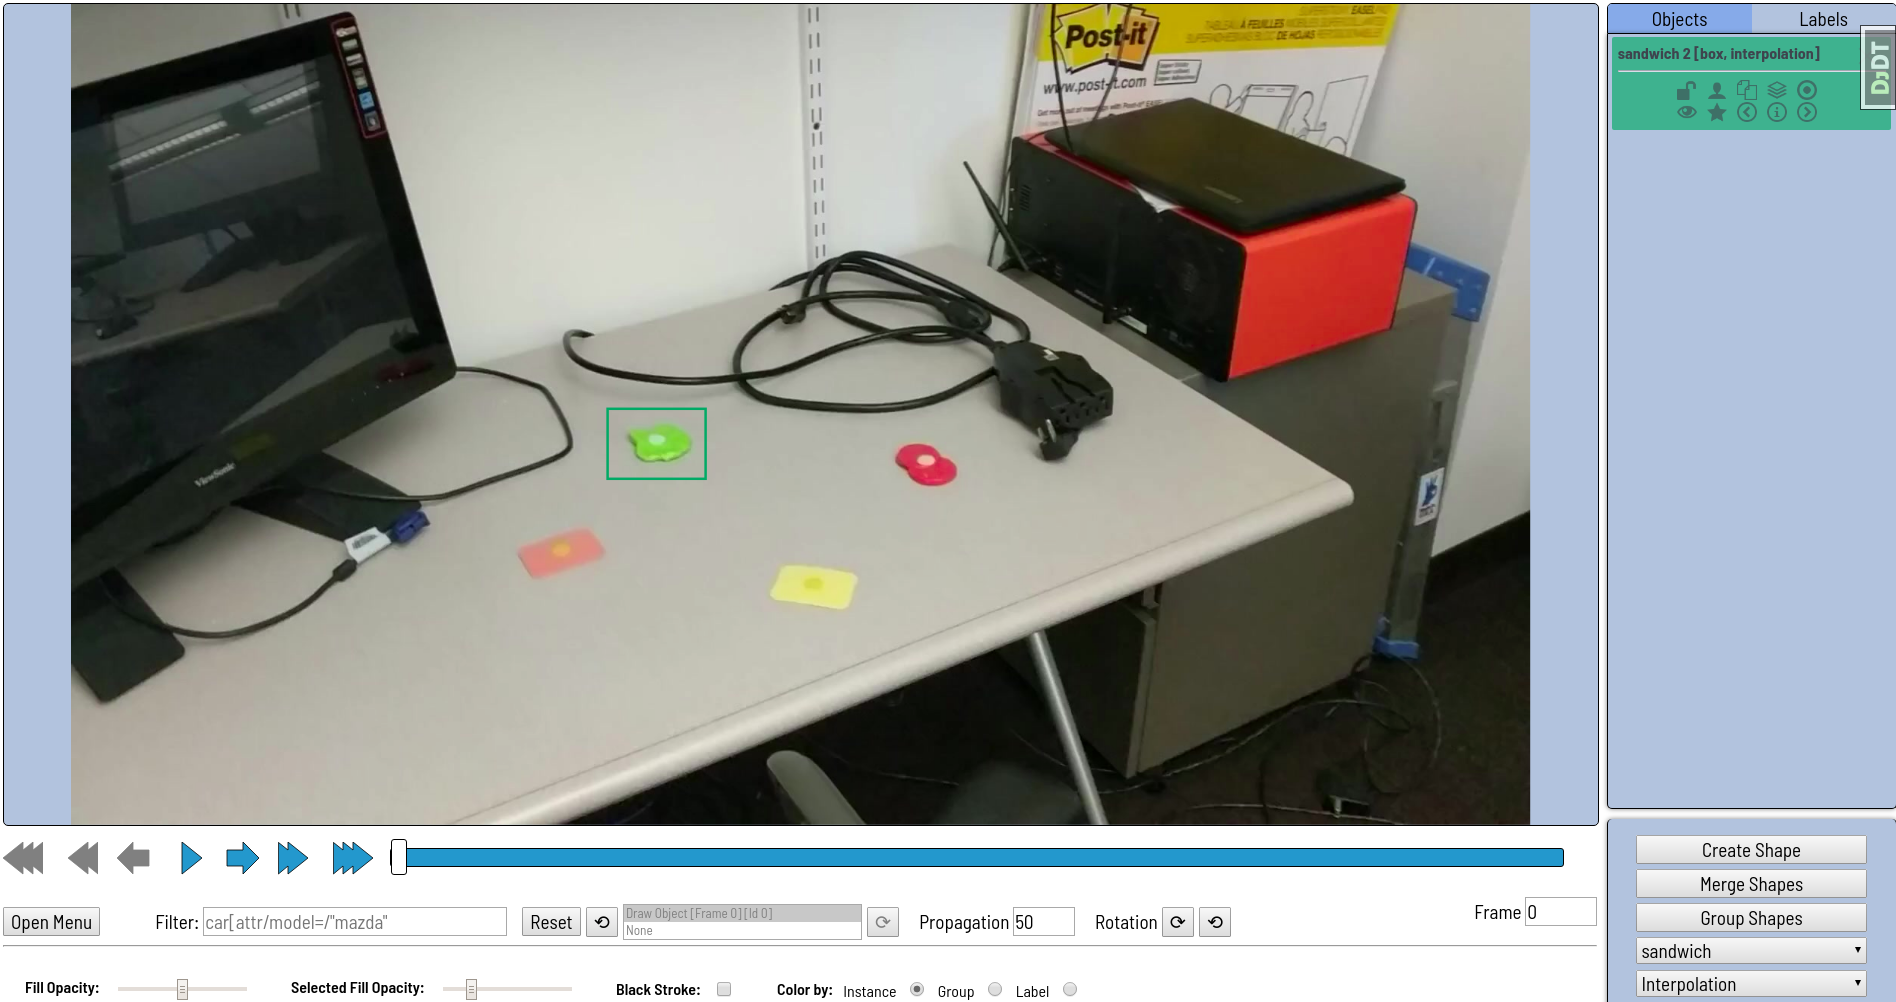
\includegraphics[width=\textwidth]{FIGS/tpod-label-gui}}
    \caption{TPOD Integration of an External Labeling Tool}
  \label{figs:tpod-label-gui}
\end{figure}

With videos annotated, users can move on to create dataset for training by
selecting videos to use. TPOD performs a data cleaning and augmentation pass to
prepare a high quality training set. Due to interframe correlations, adjacent
frames within the video may appear to be very similar or even identical. These
highly correlated frames violates the indepedent and identically distributed
assumption of training data for DNNs. TPOD eliminates these near duplicate
examples, as they would increase the model biases.  Optionally, data
augmentation can be employed. It adds synthetic images, created by cutting and
pasting the object of interests on varying backgrounds, at different scales and
rotations. Such augmentation has been shown to help produce more robust object
detectors~\cite{dwibedi2017cut}.

Then, by submitting a form on the web GUI, users can launch the DNN training
process with writing a single line of code. TPOD underneath automate the
transfer learning process of a DNN model using user specified dataset. TPOD
supports several state-of-the-art object detection network for transfer
learning, including FasterRCNN-ResNet~\cite{ren2015faster}~\cite{He2016} and
SSD-MobileNet~\cite{Liu2016}~\cite{Howard2017}. These different networks exhibit
different accuracy versus speed trade-off. While FasterRCNN-ResNet achieves
higher accuracies on standard datasets, its training and inference time are
significantly longer than SSD-MobileNet. Application developers should choose
the appropriate DNN network based on their accuracy and latency constraints.
Negative examples are mined from the video background; these are parts of the
frames not included in the object bounding boxes.  The training is started as a
batch process that uses a standard, scripted learning schedule, and generates
downloadable Tensorflow model in the end. The TPOD web interface provides
training monitoring and download links for the created model files. TPOD also
provides a container image that can directly serve the downloaded model files
for inference.

Overall, TPOD can greatly reduce both the labeling effort and in-depth machine
learning knowledge needed to effectively train and deploy a DNN-based detector.
The initial prototype of TPOD has been used by researchers and students to build
wearable cognitive assistance. For example, a group of master students in CMU
mobile and pervasive computing class successfully used TPOD to build an
assistant for using Automated External Defibrillator (AED) machines.

\subsection{TPOD Case Study for Cooking Application}

To quantify how much TPOD can help reduce laboring efforts in training object
detectors, we conduct a case study to train detectors for the Cooking cognitive
assistance~\cite{chen2018application}. We trained object detectors for 9
components of a toy sandwich, including bread, ham, lettuce, cucumber, cheese,
half sandwich, ham wrong state, tomato, and full sandwich. We collected 53 short
training videos, annotated all videos, and trained object detectors all with
TPOD.

In total, we collected 21218 frames with the videos. When using TPOD's labeling,
we only manually labeled 91 frames. The rest of frames are automatically labeled
by TPOD's tracking component. The total labeling session lasted 80 minutes. The
total number of frames used for training is 21013, because of data set
optimization. We fine-tuned from a FasterRCNN-VGG network. The finetuning
process took 54 minutes to finish on a NVIDIA K40c GPU.


\subsection{TPOD Architecture}

\begin{figure}[]
  \hspace{-.1in}
    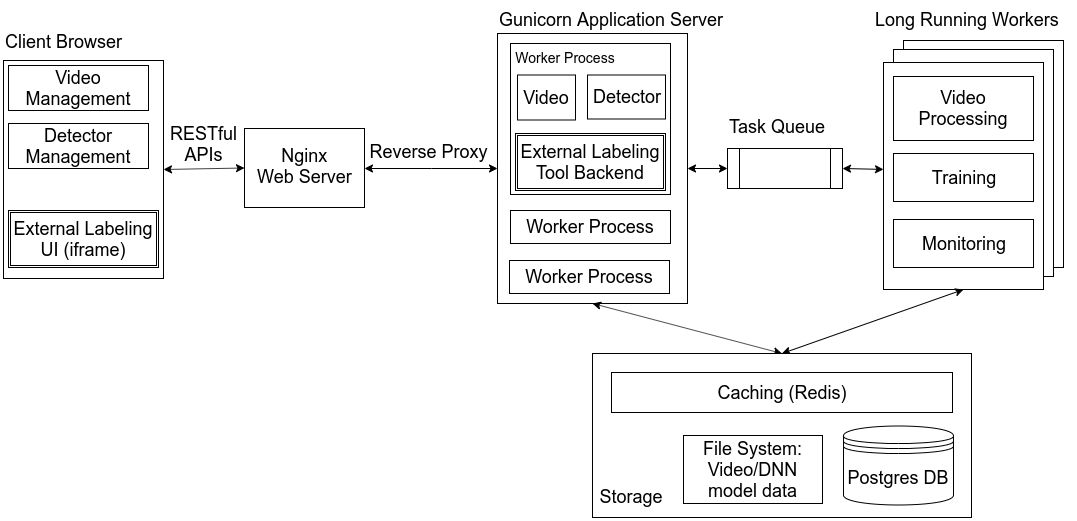
\includegraphics[width=1.1\textwidth]{FIGS/tpod-arch}
    \caption{TPOD Architecture}
  \label{figs:tpod-arch}
\end{figure}

TPOD adopts a Model-View-Controller (MVC) design for web
applications~\cite{krasner1988description}. Figure~\ref{figs:tpod-arch} shows
TPOD architecture. TPOD frontend handles UI logic and is built using React, a
declarative, efficient, and flexible JavaScript library for creating user
interface~\cite{staff2016react}. React enable TPOD frontend code to be modular
and reusable. The frontend has three major components: video management,
detector management, and an external labeling tool. TPOD integrate the labeling
tool CVAT~\cite{cvat2019} into its frontend through embedding via an iframe. The
embedding of an labeling tool directly into the GUI unifies the workflow to
eliminate users' need to set up and use another piece of software. TPOD frontend
communicates with the backend using a set of RESTful
apis~\cite{richardson2008restful}, centered around \textit{Video} and
\textit{Detector} resources. 

TPOD backend is developed using the Django web
framework~\cite{holovaty2009definitive} and served with Nginx web
server~\cite{nedelcu2010nginx} and Gunicorn application
server~\cite{gunicorn2017http}. The backend implements the RESTful apis to
create, read, update, and delete \textit{Video} and \textit{Detector} resources.
It also interface with the external labeling tool CVAT's backend to read and
write annotations. Long running background jobs, such as DNN model training and
video extraction is processed asynchronously using a task queue and
long running worker processes. Metadata about videos and DNN models are stored
in a relational database while large binary files, such as video files and
trained DNN model weights are stored in the file system. An in-memory caching
layer on top of the file system and database is created using key-value store
Redis. The entire application is containerized and can be deployed easily onto
bare-metal or virtualized environment.

One key design choice of TPOD is to be extensible for new DNN architectures.
TPOD provide a standard interface, shown in
Figure~\ref{figs:tpod-provider-interface} to add new DNNs implementation for
transfer learning. TPOD refers to these DNN implementations as DNN
\textit{Providers}. Providers do no need to know anything else about TPOD and
only need to implement the Provider interface to be integrated and used. The
built-in \textit{Provider} is Tensorflow's object detection API, which supports
transfer learning for a wide set of object detectors~\cite{tfod2019}. 


\begin{algorithm} 
% \addcontentsline{TPOD Provider Interface}{algorithm}{TPOD Provider Interface}
\SetAlgoLined
 property \textbf{training\_configurations}: user customizable hyperparameters\;
 \textbf{init(dnn\_type, training\_set, output\_directory)}: initialization\;
 \textbf{train(training\_configurations)}: launch training\;
 \textbf{export()}: export trained models\;
 \textbf{visualization()}: monitor training process\;
\caption{TPOD Provider Interface}
\label{figs:tpod-provider-interface}
\end{algorithm}